\section{Studies of noise peak movement under temperature variation}
Since we are using SiPMs with a sensitive area of $3\times3\,\mathrm{mm}$ we discovered a clipping in our frontend electronics due to higher signals. Therefore we had to set down the amplification factor. This implicates that individual p.e. peaks were not observable anymore. Therefore the possiblity to regulated the bias voltage on temperature variation by measuring the asymmetry of the edges of the first p.e. to keep it on a constant value could not be realized in that way. But a implementation of this algorithm on the entire noise peak could be possible which leads to these studies.

\subsection{Testsetup}
To measure the movement of the noise peak under temperature variation a prototyp frontend without scintillator was put in a cooling box which could be regulated with the temperature device located between the two SiPMs. The bias voltage supplied to the SiPM was fixed to a constant value. The fingerspectra based on the peakheights was collected from pulses taken with an FADC. Thereby the peakheights were defined as the potential difference between the pulse maximum and the average baseline. The FADC was triggers itselves on pulses over $0.5\,\mathrm{p.e.}$. To avoid influence from pedestals only one SiPM-Channel was regarded. To analyse the peak a fit of an exponentially modified gaussian distribution was used due to best match to the shape.

\subsection{Results}
As one can see in figure \ref{NoiseMove} the mean of the noise peak shifts linear to smaller peakheights with increasing temperature based on the decreasing overvoltage. Also the peak width gets smaller because the gain drops with the decreasing overvoltage. Based on this it is possible to adjust the bias voltage by the movement of the noise peak.
\begin{figure}[h]
	\centering
	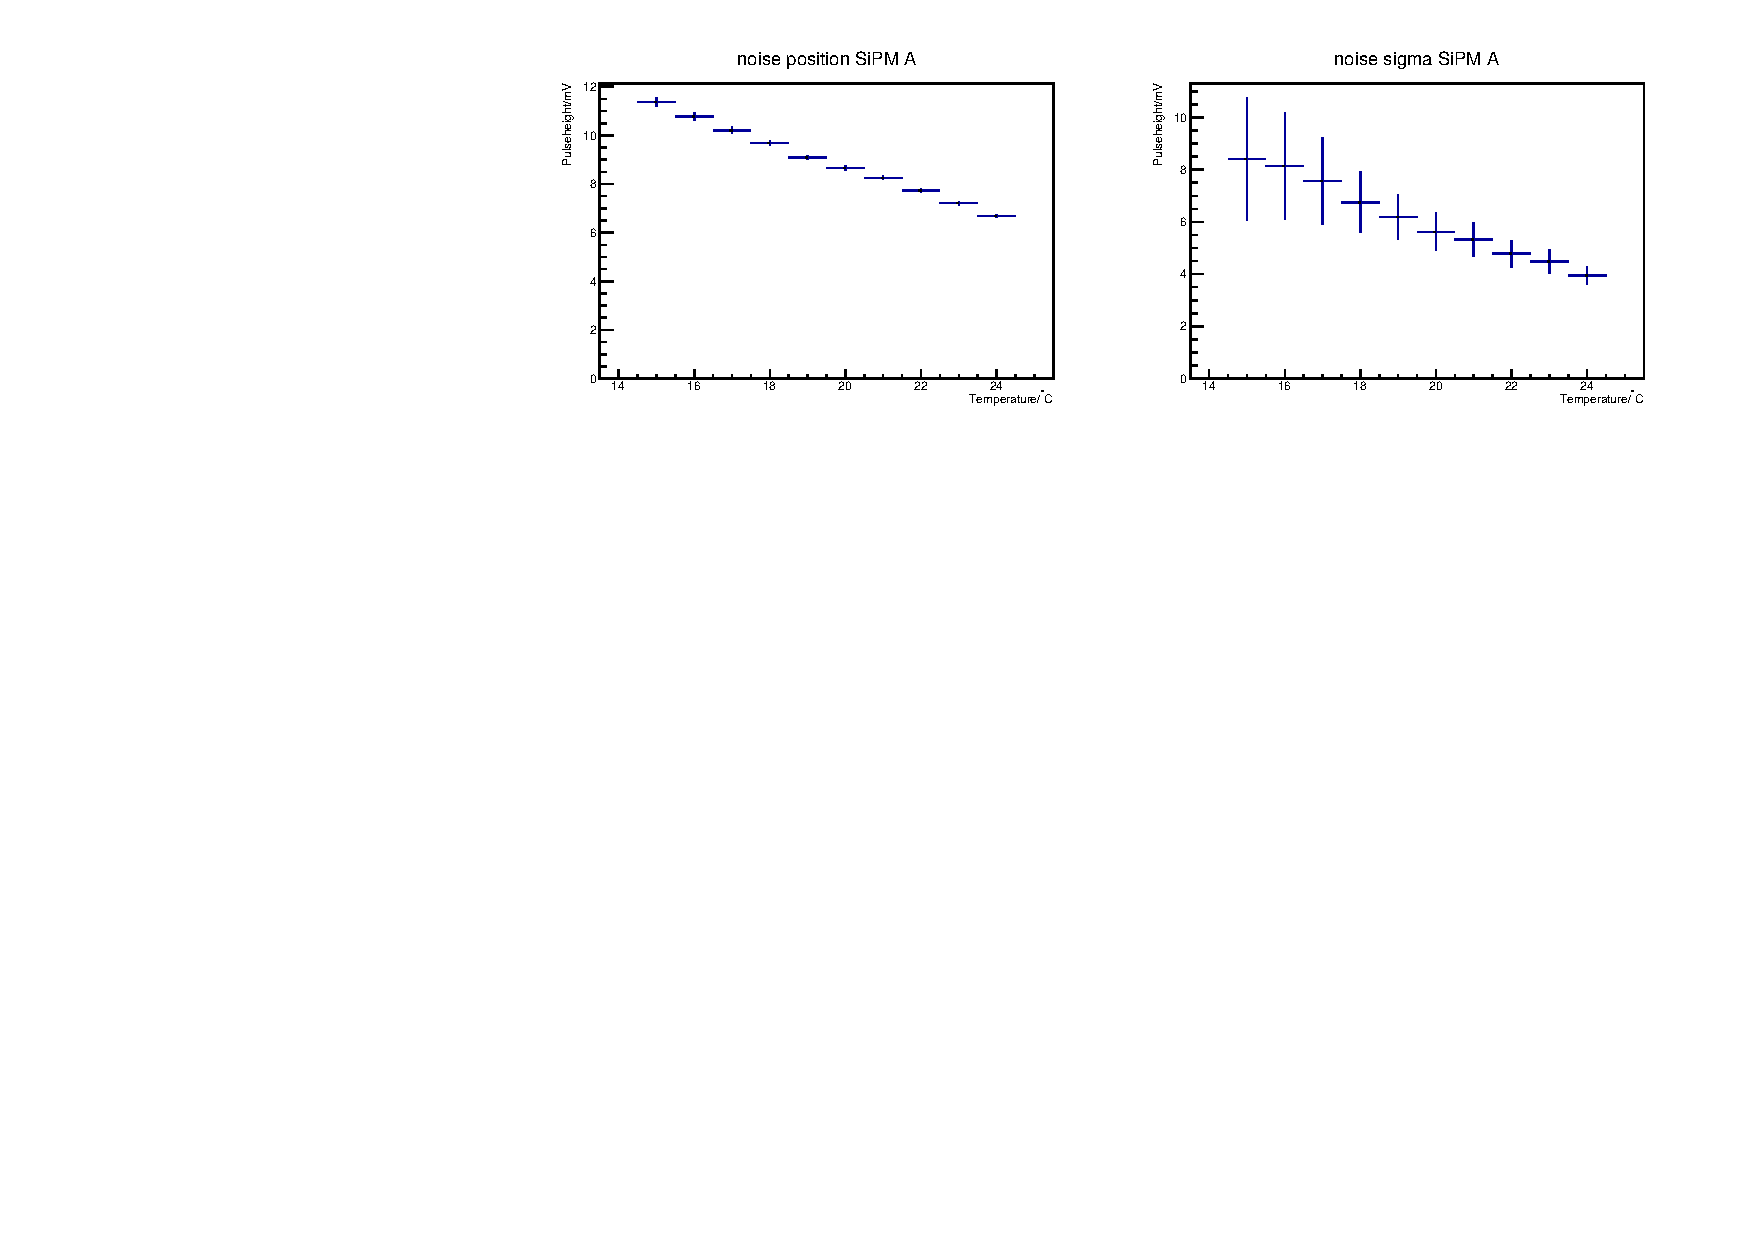
\includegraphics[width = .99\textwidth]{Figures/radermacher/result_ExpGauOnlySipmATriggerNEW.pdf}
	\caption{measurement of noise peak movement}
	\label{NoiseMove}
\end{figure}
